\documentclass{resume}

\begin{document}

\fontfamily{ppl}\selectfont

\noindent
\begin{tabularx}{\linewidth}{@{}m{0.8\textwidth} m{0.2\textwidth}@{}}
{
    \Large{Vladislav Khokhlov} \newline
    \small{
        \clink{
            \href{mailto:entergro@gmail.com}{entergro@gmail.com} \textbf{·} 
            {\fontdimen2\font=0.75ex +7 999 965 8854} 
            \textbf{·} 
            \href{https://entergro.me}{entergro.me}
        } \newline
        Moscow, Russia
    }
} & 
{
    \hfill
    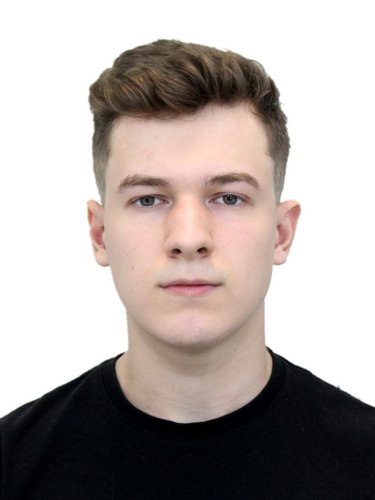
\includegraphics[width=2.8cm]{images/gr.png}
}
\end{tabularx}
\begin{center}
\begin{tabularx}{\linewidth}{@{}*{2}{X}@{}}
% left side %
{
    \csection{EXPERIENCE}{\small
        \begin{itemize}
            % item 1 %
            \item \frcontent{Orion (last MERA)}{Junior Software Engineer - Nizhniy Novgorod}{C/C++ developer. Worked with the SS7 stack of the OSI model.}{March 2019 - August 2019}
        \end{itemize}
    }
    \csection{EDUCATION}{\small
        \begin{itemize}
            % item 1 %
            \item \frcontent{Bachelor CS, GPA: 7.8/10}{Higher School of Economics}{}{2019-2023}
        \end{itemize}
    }
        \csection{ABOUT}{\small
            \begin{itemize}
                I have experience working in a team and a large project. I know Python and C++. Preferred direction: backend. I am studying in the direction related to machine learning/distributed systems. Ready to work part-time.
            \end{itemize}

    }
}
% end left side %
& 
% right side %
{
    \csection{SKILLS}{\small
        \begin{itemize}
            \item \textbf{Technologies} \newline
            {\footnotesize C++, C, Python, Django (+DRF), FastAPI, Flask, Git, aiohttp}{}{}
            \item \textbf{Patterns \& Practices} \newline
            {\footnotesize Object Oriented Programming, Functional  Programming}
            \item \textbf{Project Management} \newline
            {\footnotesize Agile, Scrum, Kanban, Yandex Tracker}
        \end{itemize}
    }
}
\end{tabularx}
\end{center}
\end{document}